\documentclass{beamer}
\usepackage[utf8]{inputenc}
\usepackage[magyar]{babel}
\usepackage{t1enc}
\usepackage{multirow}
\usepackage{tikz}
\usetikzlibrary{shapes, calc, positioning}
\mode<presentation>
{
	\usetheme{Frankfurt}
	\usecolortheme{wolverine}
	\usefonttheme{structurebold}
	\setbeamertemplate{navigation symbols}{}
	\setbeamertemplate{caption}[numbered]
}
\makeatletter
\DeclareRobustCommand{\rgbdddot}[1]{%
	{\mathop{\kern\z@#1}\limits^{%
			\vbox to-1.55\ex@{%
				\kern-\tw@\ex@
				\hbox{
					\normalfont
					\kern0.0em\textcolor{red}{.}
					\kern-0.5em\textcolor{green}{.}
					\kern-0.5em\textcolor{blue}{.}
				}
				\vss
			}
		}
	}
}
\makeatother

\title{Modern sorrend-független átlátszósági technikák}
\subtitle{Önálló  laboratórium}
\author{Cuellar-Magyar Ádám}

\begin{document}
	
\begin{frame}
	\titlepage
\end{frame}
	
\section{Bevezető}
\subsection{Bevezető}
\begin{frame}{Motiváció}{A klasszikus A over B operátor}
	A probléma a következő:
	\begin{itemize}
		\item Az áttetsző felületek átfedéséből eredő látható szín függ a felületek mélységi sorrendjétől. Ez fontos szerepet játszik a térlátásban.
		\item A mélység tesztelés időbeli sorrendje is meghatározó a helyes kitakarásban, ahogy az \aref{img:invisglass}.~ábrán látható.
		\item Túl költséges a képtér objektumait képkockánként mélység szerint sorba rendezni.
		\item Alakzatok metszése esetén pixelenkénti sorrend meghatározása szükséges.
	\end{itemize}
\end{frame}

\begin{frame}{Motiváció}{A klasszikus A over B operátor}
	\begin{figure}
		\centering
		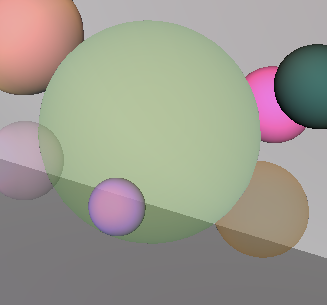
\includegraphics[scale=0.4]{invisglass.png}
		\caption{Helytelen rajz sorrend eredménye. A zöld gömb helyesen mutatja a lila gömböt mögötte, de kitakarja a rózsaszín és barna gomböket.}
		\label{img:invisglass}
	\end{figure}
\end{frame}

\section{Régi technikák}
\subsection{Depth Peeling}
\begin{frame}{Depth Peeling}
	\begin{itemize}
		\item Ez az OIT technika a képteret több ``rétegre'' osztja fel, majd ezeket a tárolt $\alpha$-érték szerint összekeveri a kimeneti kép elkészítéséhez.
		\item Az első réteg eltárolja a nézőpontból látható $RGB\alpha$ értékeket, a második mindazt, amit az első kitakart, és így tovább. Ily módon ``implicit'' sorrendezéssel pontos eredményt állít elő $n$ rétegből.
		\item A többmenetes rajzolás költsége összetettebb jelenetek esetén eltörpül a sorbarendezés (idő-)költsége melett.
	\end{itemize}
		
\end{frame}
	
\begin{frame}{Depth Peeling}
	\begin{figure}[bpl]
		\centering
		\begin{tikzpicture}[rectangle, minimum size = 20pt, node distance=2cm]
			\node[] (0) {
				
\includegraphics[scale=0.05]{camera-equipment-image-svgrepo-com.eps}
			};
			\node[draw, right of = 0, label=below:1.réteg] (1) {$RGB\alpha$};
			\draw[->] (0) to node[above] {} (1);
			\node[right of = 1] (2) {\ldots};
			\draw[->] (1) to node[above] {} (2);
			\node[draw, right of = 2, label=below:$n$. réteg] (3) {$RGB\alpha$};
			\draw[->] (2) to node[above] {} (3);
			\label{fig:depthpeeling}
		\end{tikzpicture}
		\caption{A képteret rajzolással sorbarendezzük, sorbarendezéses rajzolás helyett.}
	\end{figure}
	\begin{figure}[bpr]
		$$	\LARGE \rgbdddot{C_{A over B}} = \rgbdddot{C_A} + (1 - \alpha_A) \cdot \rgbdddot{C_B} $$
		\caption{A keverés maga egyszerű.}
	\end{figure}
\end{frame}

\begin{frame}{Depth Peeling}
	Az eljárás teljesítménye javítható különféle módokon, például:
	\begin{itemize}
		\label{list:depthpeelvariants}
		\item Az átlátszatlan objektumok mélységének egy külön előmenetbeli\index{prepass, előmenet} felrajzolása egy textúrába\index{textúra}, amelyet felhasználhatunk a képtér hátulról előre haladó hámozásakor, így nem kell az algoritmust futtatni olyan fragmenseken\index{fragment, fragmens} amelyek nem is láthatók.
		\item Az $n$ réteg külön-külön tárolása helyett létrehozunk egy gyüjtő- és egy pásztázó framebuffer-t\index{framebuffer}. A pásztázó buffer tartalma közvetlen a képrajzolás után belekeverhető a gyüjtőbe. Ez a megoldás jól kombinálható az előzővel, ugyanis ehhez is hátulról előre kell bejárni a képteret.
	\end{itemize}
\end{frame}
	
\section{Modern technikák}
\subsection{Approximációs technikák}
\begin{frame} {Moment-based OIT}
	\begin{itemize}
	\item A MBOIT egy relatíve új technika, amely a képtér pixelenkénti láthatósági függvényére ad megközelítést vagy hatványos, vagy akár trigonometrikus momentumok használatával.
	
	\item A művelet két menetet követel meg, először a jelenet láthatósági függvényeinek meghatározásához, másodszor az átlátszó felületek összeállításához.
	\end{itemize}
\end{frame} 

%\begin{frame} {Moment-based OIT}
%	A láthatóság logaritmusával, az elnyeléssel számolunk.
%	$$A(z_f) := -\ln\,T(z_f) = \sum_{\substack{l=0\\z_l<z_f}}^{n-1}-\ln(1-\alpha_l)$$
%	Szükség van egy momentum-generáló függvényre: $\boldsymbol{b} : [-1,1] \rightarrow \mathbb{R}^{m+1}$. Így a következő képlettel a vizsgált pixelbeli teljes láthatósági függvény megközelítése hatékonyan eltárolható.
%	$$b:=\mathcal{E}_Z(\boldsymbol{b}):=\sum_{l=0}^{n-1}-\ln(1-\alpha_l)\cdot\boldsymbol{b}(z_l)$$
%	Kompozíció idején visszanyerhetjük a láthatósági függvényt:
%	$$\sum_{l=0}^{n-1}L_l\cdot\alpha_l\cdot exp(-A(z_f,\boldsymbol{b},\beta))$$
%\end{frame}

\begin{frame}{Wavelet OIT}
	Lényeges különbségek:
	\begin{itemize}
		\item Ez a technika nem törekszik fizikai szimuláció szintű pontosságot produkálni, ellenkezőleg éppen az emberi észlelés sajátosságaira hagyatkozik, hogy végül egy ``hihetőbb'' képet alkosson, az átlátszóság bármilyen alkalmazásában, legyen az köd vagy haj.
		\item A láthatósági függvényt momentumok helyett wavelet-ekkel tárolja, amiknek köszönhetően pontosabb becslést tudunk megadni a láthatósági függvényre, kisebb memóriaigénnyel.
	\end{itemize}
\end{frame}

\section{Saját munka}
\subsection{keret}
\begin{frame}{Keret}
	\begin{itemize}
		\item A demó programhoz sok inspirációt vettem a 3D Grafikus Rendszerek tárgy laborjain használt kódból. \`Igy minden elemet felparaméterezhető objektumokból állíthattam össze.
		\item A Grafikus könyvtár OpenGL 4.6.0
	\end{itemize}
\end{frame}
\subsection{nehézségek}
\begin{frame}{Nehézségek}
	\begin{itemize}
		\item A keretet a félév nagy részében ``vakon'' fejlesztettem, így kellemetlen volt felfedezni, hogy a transzformációs mátrixaimat rossz sorrendben szorzoztam össze, de végül konzulensemmel kibogoztuk őket.
		\item A legújabb, jelenleg is fennálló probléma az objektumok árnyalásában jelenik meg, egy ``tigrisminta''~-szerű árnyékban [\ref{img:tigerprint}] minden áttetsző objektumon, de csak bizonyos irányokból, és csak ha távol van a kamera fókuszától.
	\end{itemize}
\end{frame}

\begin{frame}{Egy kép mint száz szó}
	\begin{figure}[ht]
		\begin{minipage}[b]{0.45\linewidth}
			\centering
			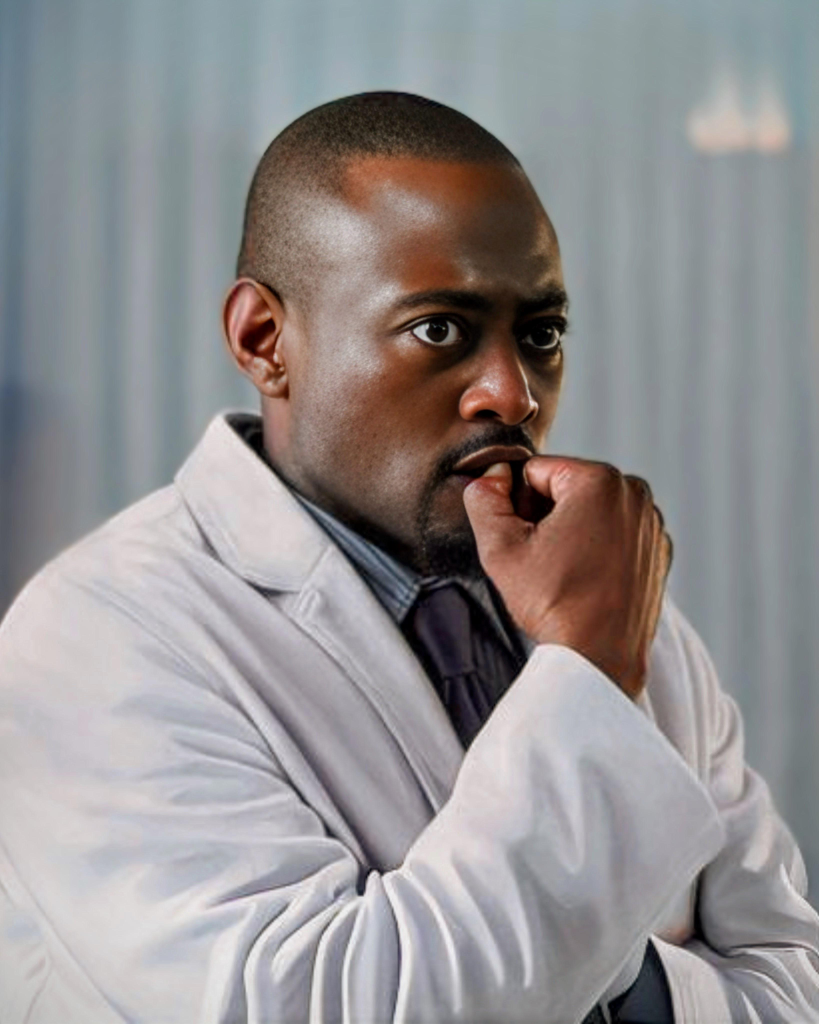
\includegraphics[width=\textwidth]{vex.png}%
		\end{minipage}
		\hspace*{0.5cm}
		\begin{minipage}[b]{0.45\linewidth}
			\centering
			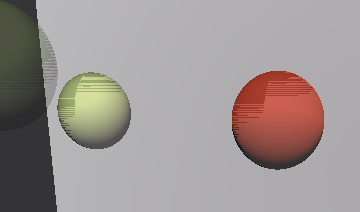
\includegraphics[width=\textwidth]{tigerprint.png}%
			\label{img:tigerprint}
		\end{minipage}
	\end{figure}
\end{frame}

\subsection{kitekintés}
\begin{frame}{Mi következik?}
		Természetesen az MBOIT és WOIT technikák.
		
		Szakdolgozathoz pedig:
	\begin{itemize}
		\item A WOIT kutatás szerzőinek felvetése nyomán keresek egy egymenetes implementációt a WOIT algoritmushoz, ha létezhet ilyen~\dots
		\item \dots~vagy ezt kibővítem, hogy árnyékokkal is működjön\dots
	\end{itemize}
\end{frame}
\begin{frame}
	\huge \usebeamerfont{title}{Köszönöm szépen a figyelmet!}
\end{frame}
\end{document}